\documentclass{article}
\usepackage{xcolor}
\usepackage{titleps}
\usepackage[letterpaper, margin=0.95in]{geometry}
\usepackage{url}
\usepackage{amsmath}
\usepackage{amssymb}
\usepackage{wrapfig}
\usepackage{float}
\usepackage{mathtools}
\usepackage{enumitem}
\usepackage{tabu}
\usepackage{parskip}
\usepackage{natbib}
\usepackage{listings}

\usepackage[many]{tcolorbox}
\usepackage{minted}
\setminted[python]{
	% frame=single,
	% linenos,
    xleftmargin=0.475em,
    baselinestretch=1.2,
}
% https://tex.stackexchange.com/a/569249
\setcounter{secnumdepth}{5}
\setcounter{tocdepth}{5}
\makeatletter
\newcommand\subsubsubsection{\@startsection{paragraph}{4}{\z@}{-2.5ex\@plus -1ex \@minus -.25ex}{1.25ex \@plus .25ex}{\normalfont\normalsize\bfseries}}
\newcommand\subsubsubsubsection{\@startsection{subparagraph}{5}{\z@}{-2.5ex\@plus -1ex \@minus -.25ex}{1.25ex \@plus .25ex}{\normalfont\normalsize\bfseries}}
\makeatother

\usepackage{hyperref}
\usepackage[color=red]{todonotes}
\usepackage{forest}
\definecolor{light-yellow}{HTML}{FFE5CC}

\newpagestyle{ruled}
{\sethead{CMU 16-831}{Introduction to Robot Learning }{Fall 2026}\headrule
  \setfoot{}{}{}}
\pagestyle{ruled}

\renewcommand\makeheadrule{\color{black}\rule[-.75\baselineskip]{\linewidth}{0.4pt}}
\renewcommand*\footnoterule{}

\newtcolorbox[]{answer}[1][]{
    % breakable,
    enhanced,
    nobeforeafter,
    colback=white,
    title=Your Answer,
    sidebyside align=top,
    box align=top,
    #1
}



\begin{document}

\lstset{basicstyle = \ttfamily,columns=fullflexible,
backgroundcolor = \color{light-yellow}
}

\begin{centering}
    {\Large Assignment 2: Policy Gradient} \\
    \vspace{.25cm}
    % \textbf{Due September 13, 11:59 pm} \\
\end{centering}
\vspace{0.25cm}

\textbf{Andrew ID:} \texttt{mlin4} \\
\textbf{Collaborators:} \texttt{Claude (used for scripting experiments in parallel)}\\ 
\textbf{NOTE:} Please do \textbf{NOT} change the sizes of the answer blocks or plots.

\setcounter{section}{4}
\section{Small-Scale Experiments (7.5 Pts)}

\subsection{Experiment 1 (Cartpole) -- \lbrack4.5 points total\rbrack}

\subsubsection{Configurations}
\begin{answer}[title=Q5.1.1,height=6cm,width=\linewidth]
\begin{minted}
[framesep=2mm, fontsize=\scriptsize, breaklines]
{bash}
python rob831/scripts/run_hw2.py --env_name CartPole-v0 -n 150 -b 1500 \
    -dsa --exp_name q1_sb_no_rtg_dsa

python rob831/scripts/run_hw2.py --env_name CartPole-v0 -n 150 -b 1500 \
    -rtg -dsa --exp_name q1_sb_rtg_dsa

python rob831/scripts/run_hw2.py --env_name CartPole-v0 -n 150 -b 1500 \
    -rtg --exp_name q1_sb_rtg_na

python rob831/scripts/run_hw2.py --env_name CartPole-v0 -n 150 -b 6000 \
    -dsa --exp_name q1_lb_no_rtg_dsa

python rob831/scripts/run_hw2.py --env_name CartPole-v0 -n 150 -b 6000 \
    -rtg -dsa --exp_name q1_lb_rtg_dsa

python rob831/scripts/run_hw2.py --env_name CartPole-v0 -n 150 -b 6000 \
    -rtg --exp_name q1_lb_rtg_na
\end{minted}
\end{answer}

\subsubsection{Plots}

\subsubsubsection{Small batch -- \lbrack1 points\rbrack}
\begin{answer}[title=Q5.1.2.1,height=9.5cm,width=\linewidth]
\centering
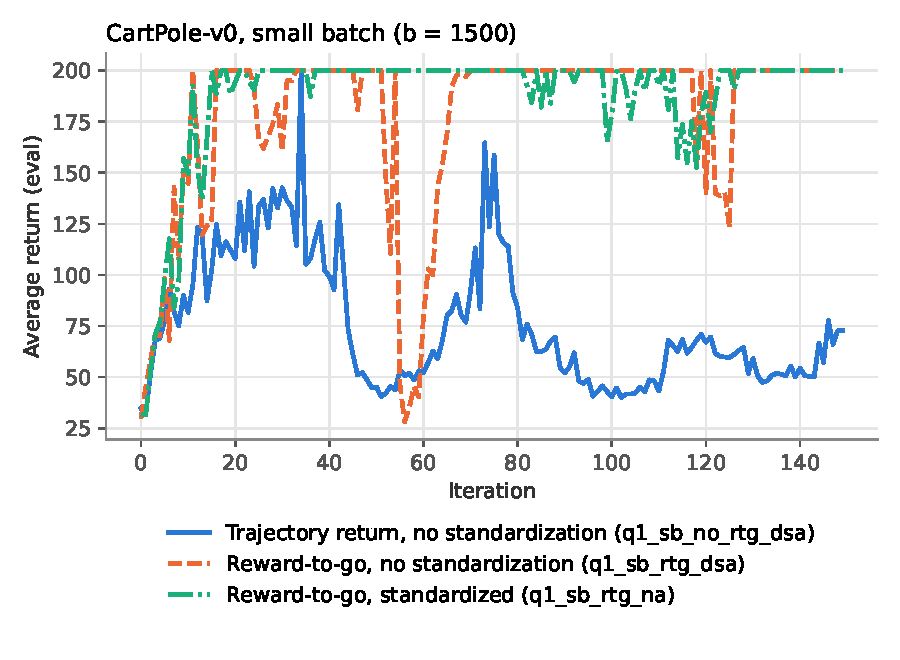
\includegraphics[height=8cm]{figures/q1_sb.pdf}
\end{answer}

\subsubsubsection{Large batch -- \lbrack0.5 points\rbrack}
\begin{answer}[title=Q5.1.2.2,height=9.5cm,width=\linewidth]
\centering
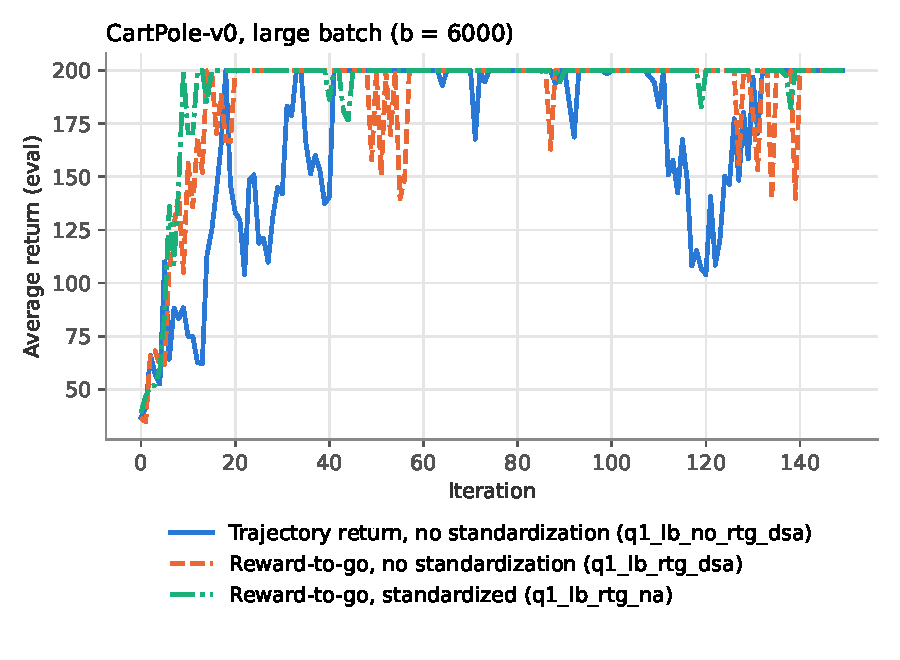
\includegraphics[height=8cm]{figures/q1_lb.pdf}
\end{answer}

\subsubsection{Analysis}

\subsubsubsection{Value estimator -- \lbrack1 points\rbrack}
\begin{answer}[title=Q5.1.3.1,height=4cm,width=\linewidth]
Both graphs suggest that reward-to-go performs significantly better than the trajectory-centric method.
\end{answer}

\subsubsubsection{Advantage standardization -- \lbrack1 points\rbrack}
\begin{answer}[title=Q5.1.3.2,height=4cm,width=\linewidth]
Advantage standardization seems to offer a modest performance improvement. Comparing the two reward-to-go runs, the run that uses advantage standardization reaches a return of 200 faster and has less severe dips in reward after capping out.
\end{answer}

\subsubsubsection{Batch size -- \lbrack1 points\rbrack}
\begin{answer}[title=Q5.1.3.3,height=4cm,width=\linewidth]
Increased batch size seems to offer benefits both for the trajectory-based and the reward-to-go methods. The trajectory-based method manages to make it to a reward of 200 after increasing the batch size and the reward-to-go methods have less severe dips in reward after capping out in the larger batch experiments.
\end{answer}

\subsection{Experiment 2 (InvertedPendulum) -- \lbrack3 points total\rbrack}

\subsubsection{Configurations -- \lbrack1 points\rbrack}
\begin{answer}[title=Q5.2.1,height=10cm,width=\linewidth]
\begin{minted}
[framesep=2mm, fontsize=\scriptsize, breaklines]
{bash}
JOBS=${JOBS:-20}
BATCHES=(100 300 500 1000 3000 5000)
LRS=(0.005 0.01 0.02 0.03 0.05)

mkdir -p logs_q2

for b in "${BATCHES[@]}"; do
  for r in "${LRS[@]}"; do
    echo "$b $r"
  done
done | xargs -P "$JOBS" -n 2 sh -c '
  b=$0; r=$1
  OMP_NUM_THREADS=1 MKL_NUM_THREADS=1 python rob831/scripts/run_hw2.py --env_name InvertedPendulum-v4 \
    --ep_len 1000 --discount 0.92 -n 100 -l 2 -s 64 -b "$b" -lr "$r" -rtg -ngpu \
    --exp_name "q2_b${b}_r${r}" > "logs_q2/q2_b${b}_r${r}.log" 2>&1
  echo "finished b=$b r=$r (exit $?)"'
\end{minted}
\end{answer}

\subsubsection{smallest \textbf{b*} and largest \textbf{r*} (same run) -- \lbrack1 points\rbrack}
\begin{answer}[title=Q5.2.2,height=4cm,width=\linewidth]
$b* = 500$ and $r* = 0.03$
\end{answer}

\subsubsection{Plot -- \lbrack1 points\rbrack}
\begin{answer}[title=Q5.2.3,height=10cm,width=\linewidth]
\centering
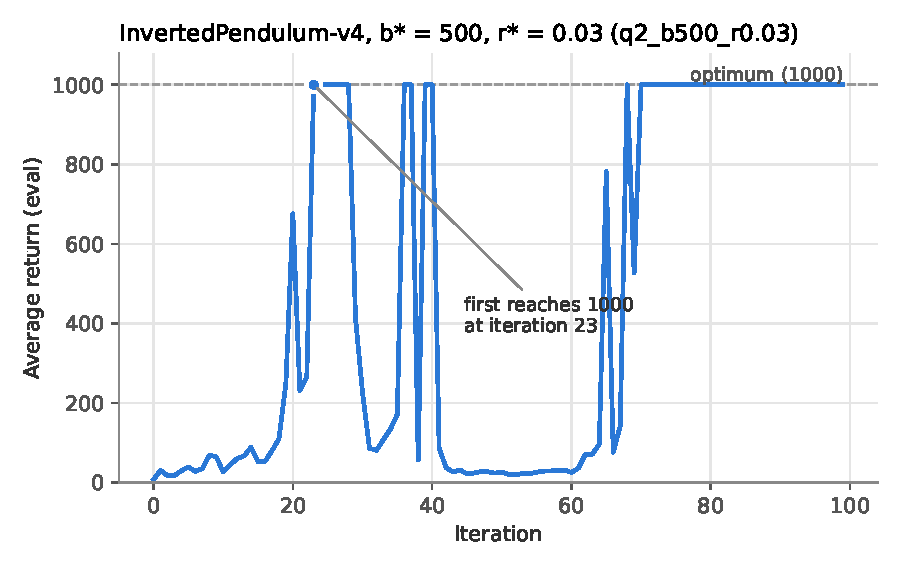
\includegraphics[height=8cm]{figures/q2.pdf}
\end{answer}

\setcounter{section}{6}
\section{More Complex Experiments (4.5 Pts)}

\subsection{Experiment 3 (LunarLander) -- \lbrack1 points total\rbrack}

\subsubsection{Configurations}
\begin{answer}[title=Q7.1.1,height=6cm,width=\linewidth]
\begin{minted}
[framesep=2mm, fontsize=\scriptsize, breaklines]
{bash}
python rob831/scripts/run_hw2.py \
    --env_name LunarLanderContinuous-v2 --ep_len 1000
    --discount 0.99 -n 100 -l 2 -s 64 -b 10000 -lr 0.005 \
    --reward_to_go --nn_baseline --exp_name q3_b10000_r0.005 \
    --seed 5
\end{minted}
\end{answer}

\subsubsection{Plot -- \lbrack1 points\rbrack}
\begin{answer}[title=Q7.1.2,height=10cm,width=\linewidth]
\centering
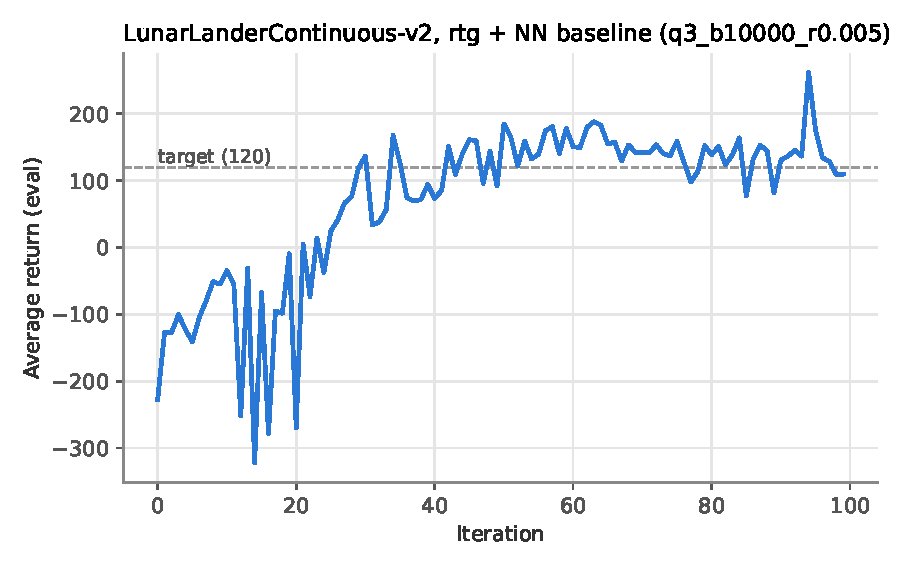
\includegraphics[height=8cm]{figures/q3.pdf}
\end{answer}

\subsection{Experiment 4 (HalfCheetah) -- \lbrack3.5 points\rbrack}

\subsubsection{Configurations}
\begin{answer}[title=Q7.2.1,height=10cm,width=\linewidth]
\begin{minted}
[framesep=2mm, fontsize=\scriptsize, breaklines, escapeinside=||, mathescape=true]
{python}
python rob831/scripts/run_hw2.py --env_name HalfCheetah-v4 --ep_len 150 --discount 0.95 -n 100 -l 2 -s 32 -b 10000 -lr 0.005 -rtg --nn_baseline -ngpu --exp_name q4_search_b10000_lr0.005_rtg_nnbaseline
python rob831/scripts/run_hw2.py --env_name HalfCheetah-v4 --ep_len 150 --discount 0.95 -n 100 -l 2 -s 32 -b 10000 -lr 0.01 -rtg --nn_baseline -ngpu --exp_name q4_search_b10000_lr0.01_rtg_nnbaseline
python rob831/scripts/run_hw2.py --env_name HalfCheetah-v4 --ep_len 150 --discount 0.95 -n 100 -l 2 -s 32 -b 10000 -lr 0.02 -rtg --nn_baseline -ngpu --exp_name q4_search_b10000_lr0.02_rtg_nnbaseline
python rob831/scripts/run_hw2.py --env_name HalfCheetah-v4 --ep_len 150 --discount 0.95 -n 100 -l 2 -s 32 -b 30000 -lr 0.005 -rtg --nn_baseline -ngpu --exp_name q4_search_b30000_lr0.005_rtg_nnbaseline
python rob831/scripts/run_hw2.py --env_name HalfCheetah-v4 --ep_len 150 --discount 0.95 -n 100 -l 2 -s 32 -b 30000 -lr 0.01 -rtg --nn_baseline -ngpu --exp_name q4_search_b30000_lr0.01_rtg_nnbaseline
python rob831/scripts/run_hw2.py --env_name HalfCheetah-v4 --ep_len 150 --discount 0.95 -n 100 -l 2 -s 32 -b 30000 -lr 0.02 -rtg --nn_baseline -ngpu --exp_name q4_search_b30000_lr0.02_rtg_nnbaseline
python rob831/scripts/run_hw2.py --env_name HalfCheetah-v4 --ep_len 150 --discount 0.95 -n 100 -l 2 -s 32 -b 50000 -lr 0.005 -rtg --nn_baseline -ngpu --exp_name q4_search_b50000_lr0.005_rtg_nnbaseline
python rob831/scripts/run_hw2.py --env_name HalfCheetah-v4 --ep_len 150 --discount 0.95 -n 100 -l 2 -s 32 -b 50000 -lr 0.01 -rtg --nn_baseline -ngpu --exp_name q4_search_b50000_lr0.01_rtg_nnbaseline
python rob831/scripts/run_hw2.py --env_name HalfCheetah-v4 --ep_len 150 --discount 0.95 -n 100 -l 2 -s 32 -b 50000 -lr 0.02 -rtg --nn_baseline -ngpu --exp_name q4_search_b50000_lr0.02_rtg_nnbaseline
\end{minted}
\end{answer}

\subsubsection{Plot -- \lbrack1 points\rbrack}
\begin{answer}[title=Q7.2.2,height=10cm,width=\linewidth]
\centering
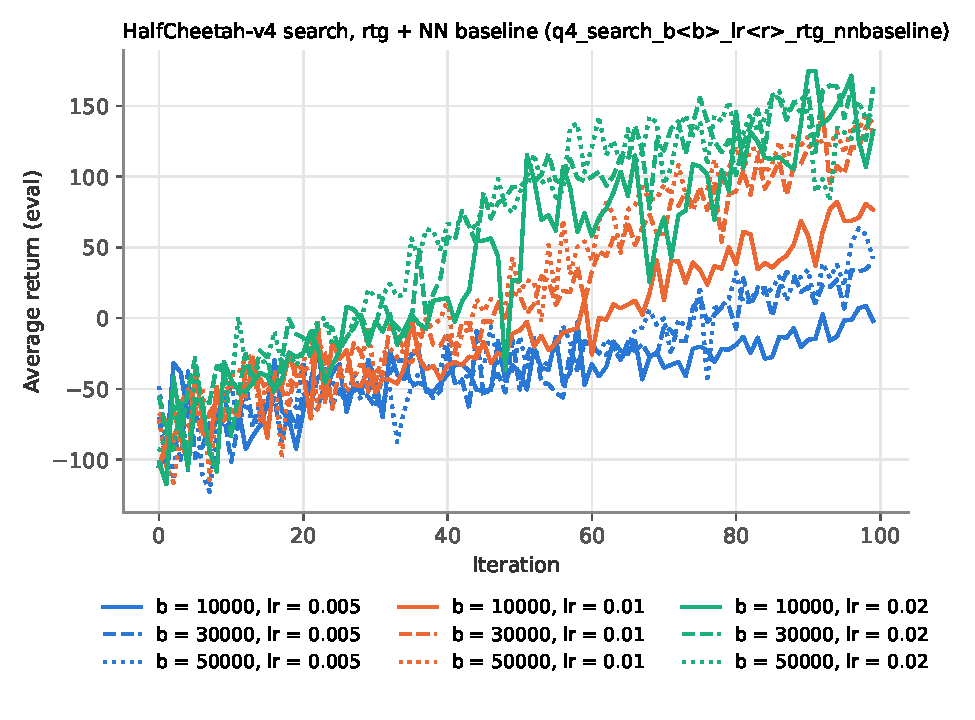
\includegraphics[height=8cm]{figures/q4_search.pdf}
\end{answer}

\subsubsection{ Optimal b* and r* -- \lbrack0.5 points\rbrack}
\begin{answer}[title=Q7.2.3,height=4cm,width=\linewidth]
$b* = 30000$ and $r* = 0.02$
\end{answer}

\subsubsection{ Plot -- \lbrack0.5 points\rbrack}
\begin{answer}[title=Q7.2.4,height=10cm,width=\linewidth]
\centering
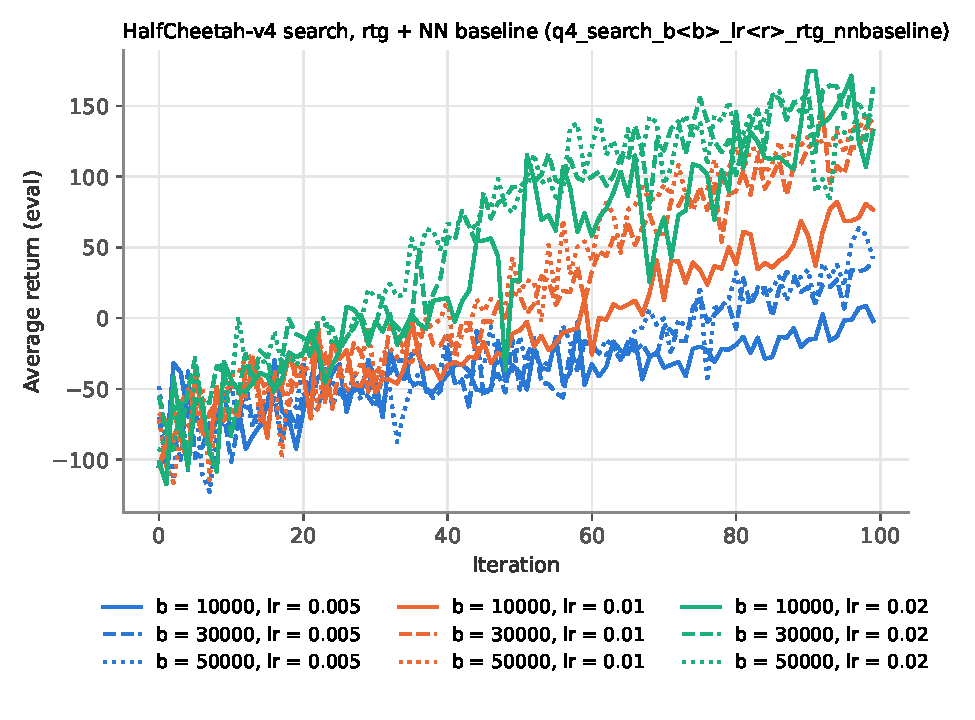
\includegraphics[height=8cm]{figures/q4_search.pdf}
\end{answer}

\subsubsection{ Describe how b* and r* affect task performance -- \lbrack0.5 points\rbrack}
\begin{answer}[title=Q7.2.5,height=4cm,width=\linewidth]
Increasing learning rate leads to a marked increase in performance when holding batch size steady for any set learning rate. Increasing the batch size doesn't seem to have a strong impact; while $b* = 10000$ lags behind for most cases, there's often only a small difference between $b* = 30000$ and $b* = 50000$.
\end{answer}

\subsubsection{Configurations with optimal b* and r* -- \lbrack0.5 points\rbrack}
\begin{answer}[title=Q7.2.6,height=6cm,width=\linewidth]
\begin{minted}
[framesep=2mm, fontsize=\scriptsize, breaklines]
{bash}
python rob831/scripts/run_hw2.py --env_name HalfCheetah-v4 --ep_len 150 --discount 0.95 -n 100 -l 2 -s 32 -b 30000 -lr 0.02 -ngpu --exp_name q4_b30000_r0.02
python rob831/scripts/run_hw2.py --env_name HalfCheetah-v4 --ep_len 150 --discount 0.95 -n 100 -l 2 -s 32 -b 30000 -lr 0.02 -rtg -ngpu --exp_name q4_b30000_r0.02_rtg
python rob831/scripts/run_hw2.py --env_name HalfCheetah-v4 --ep_len 150 --discount 0.95 -n 100 -l 2 -s 32 -b 30000 -lr 0.02 --nn_baseline -ngpu --exp_name q4_b30000_r0.02_nnbaseline
python rob831/scripts/run_hw2.py --env_name HalfCheetah-v4 --ep_len 150 --discount 0.95 -n 100 -l 2 -s 32 -b 30000 -lr 0.02 -rtg --nn_baseline -ngpu --exp_name q4_b30000_r0.02_rtg_nnbaseline
\end{minted}
\end{answer}

\subsubsection{Plot for four runs with optimal b* and r* -- \lbrack0.5 points\rbrack}
\begin{answer}[title=Q7.2.7,height=10cm,width=\linewidth]
\centering
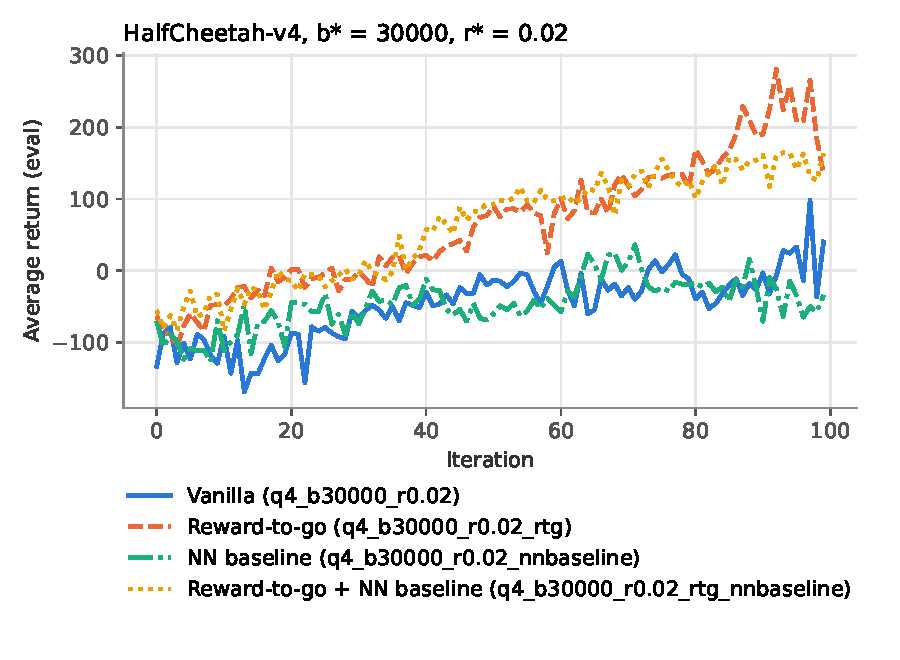
\includegraphics[height=8cm]{figures/q4_ablation.pdf}
\end{answer}

\section{Implementing Generalized Advantage Estimation (3 Pts)}

\subsection{Experiment 5 (Hopper) -- \lbrack3 points\rbrack}

\subsubsection{Configurations}
\begin{answer}[title=Q8.1.1,height=4cm,width=\linewidth]
\begin{minted}
[framesep=2mm, fontsize=\scriptsize, breaklines, escapeinside=||, mathescape=true]
{python}
python rob831/scripts/run_hw2.py --env_name Hopper-v4 --ep_len 1000 --discount 0.99 -n 300 -l 2 -s 32 -b 2000 -lr 0.001 --reward_to_go --nn_baseline --action_noise_std 0.5 --gae_lambda 0 -ngpu --exp_name q5_b2000_r0.001_lambda0
python rob831/scripts/run_hw2.py --env_name Hopper-v4 --ep_len 1000 --discount 0.99 -n 300 -l 2 -s 32 -b 2000 -lr 0.001 --reward_to_go --nn_baseline --action_noise_std 0.5 --gae_lambda 0.95 -ngpu --exp_name q5_b2000_r0.001_lambda0.95
python rob831/scripts/run_hw2.py --env_name Hopper-v4 --ep_len 1000 --discount 0.99 -n 300 -l 2 -s 32 -b 2000 -lr 0.001 --reward_to_go --nn_baseline --action_noise_std 0.5 --gae_lambda 0.99 -ngpu --exp_name q5_b2000_r0.001_lambda0.99
python rob831/scripts/run_hw2.py --env_name Hopper-v4 --ep_len 1000 --discount 0.99 -n 300 -l 2 -s 32 -b 2000 -lr 0.001 --reward_to_go --nn_baseline --action_noise_std 0.5 --gae_lambda 1 -ngpu --exp_name q5_b2000_r0.001_lambda1
\end{minted}
\end{answer}

\subsubsection{Plot -- \lbrack1 points\rbrack}
\begin{answer}[title=Q8.1.2,height=10cm,width=\linewidth]
\centering
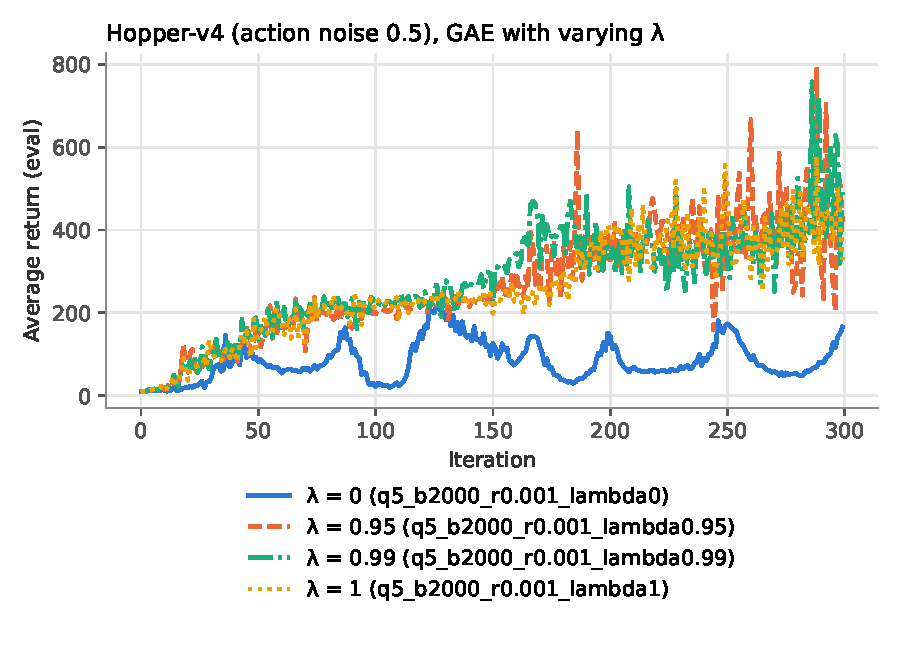
\includegraphics[height=8cm]{figures/q5.pdf}
\end{answer}

\subsubsection{Describe how $\lambda$ affects task performance -- \lbrack1.5 points\rbrack}
\begin{answer}[title=Q8.1.3,height=4cm,width=\linewidth]
$\lambda = 0$ leads to much lower performance relative to the other runs that we did. There is no notable performance difference between the three other settings of lambda that we tested. However, it is interesting to observe the bias-variance tradeoff that is discussed in the GAE paper: setting a lambda near 1 leads to much spikier lines than the $\lambda=0$ run, which is in line with the consequence of high variance when we have a high $lambda$.
\end{answer}

\subsubsection{Find one robotics paper from the last 5 years that uses policy gradients or an actor-critic method as part of its methodology. 
    In a short paragraph (4--5 sentences): (i) cite the paper, (ii) briefly describe the robot task and how reinforcement learning is used, and (iii) identify one technique from this homework (e.g., reward-to-go, a value-function baseline, or GAE) that is related to the method used in the paper. A few sentences is enough; this is not meant to be an extensive literature review  -- \lbrack0.5 points\rbrack
}
\begin{answer}[title=Q8.1.4,height=4cm,width=\linewidth]
    \textit{Learning to Walk in Minutes Using Massively Parallel Deep Reinforcement Learning}(Rudin et al.) is a paper from 2021 that was published in CoRL. The objective of the paper was to develop a quadruped robot to follow paths over rough terrain (e.g. slopes, stairs). The approach that they used was completely RL-based and train in simulation, where large quantities of "dogs" were trained alongside each other, before Sim2Real transfer and experiments in the real world. They utilize GAE in their approach and use a GAE discount factor of 0.95, which is in line with the near-one values of $\lambda$ that we tested in our experiments.
\end{answer}

\end{document}
